\documentclass[oneside,final,14pt,a4paper]{extreport}

# set the compiler XeLatex to use fontspec package
\usepackage{fontspec}

\setmainfont{Times New Roman}

\usepackage{vmargin}
\setpapersize{A4}
\setmarginsrb{2.5cm}{2.2cm}{2.2cm}{2.2cm}{0pt}{10mm}{0pt}{13mm}
\usepackage{setspace}
\sloppy
\setstretch{1.5}
\usepackage{indentfirst}
\parindent=1.25cm

%%%%% ADDED TO SUPPORT TT BOLD FACES %%%%
\DeclareFontShape{OT1}{cmtt}{bx}{n}{<5><6><7><8><9><10><10.95><12><14.4><17.28><20.74><24.88>cmttb10}{}
\renewcommand{\ttdefault}{pcr}
%%%%% END %%%%%%%%%%%%%%%%%%%%%%%%%%%%%%%
\usepackage{atbegshi,picture}
\usepackage[T1,T2A]{fontenc}
\usepackage[utf8]{inputenc}
\AtBeginShipout{\AtBeginShipoutUpperLeft{%
  \put(\dimexpr\paperwidth-1cm\relax,-1.5cm){\makebox[0pt][r]{
\includegraphics[width=3cm]{figs/inno}}}%
}}


\usepackage[english]{babel}
\usepackage[backend=biber,style=ieee,autocite=inline]{biblatex}
\bibliography{ref.bib}
\DefineBibliographyStrings{english}{%
  bibliography = {References},}
\usepackage{blindtext}


\usepackage{pdfpages}
\newenvironment{bottompar}{\par\vspace*{\fill}}{\clearpage}
\usepackage{amsmath,amsfonts}
\usepackage{url}

\usepackage{amsthm}
\newtheorem{theorem}{Theorem}
\newtheorem{corollary}{Corollary}
\newtheorem{lemma}{Lemma}
\newtheorem{proposition}{Proposition}
\theoremstyle{definition}
\newtheorem{definition}{Definition}
\theoremstyle{remark}
\newtheorem*{remark}{Remark}
\theoremstyle{remark}
\newtheorem*{example}{Example}


\usepackage{titlesec}
\usepackage{float}
\usepackage{graphicx}
\graphicspath{{figs/}} %path to images
\usepackage{array}
\usepackage{multirow,array}
\usepackage{caption}
\usepackage{subcaption}
\usepackage{hyperref}
\usepackage{paralist}
\usepackage{listings}
\usepackage{zed-csp}
\usepackage{fancyhdr}
\usepackage{csquotes}
\usepackage{color}
% \usepackage{anyfontsize}
% \usepackage{mathptmx}
% \usepackage{t1enc}

\usepackage{chngcntr}
\usepackage{upgreek}
\usepackage{bm}
\usepackage{hyperref}
\usepackage{setspace}
\usepackage{booktabs}
\usepackage{multirow}
\usepackage{longtable}
\usepackage[font=singlespacing, labelfont=bf]{caption}
\counterwithout{table}{chapter}
\renewcommand{\thetable}{\Roman{table}}
%Hints
\newcommand\pic[1]{(Fig. \ref{#1})} %Ref on figure
\newcommand\tab[1]{(Tab. \ref{#1})} %Ref on table

\setlength{\headheight}{32.0976pt}
\usepackage{enumitem}
\newlist{inlinelist}{enumerate*}{1}
\setlist*[inlinelist,1]{%
  label=(\arabic*),
}

\setcounter{secnumdepth}{4}
\captionsetup[table]{labelfont={normalfont}, name={TABLE}, labelsep={newline}}
\counterwithout{table}{chapter}
\renewcommand{\thetable}{\Roman{table}}
\setlength{\parindent}{2em}
\DeclareCaptionLabelSeparator{figSep}{.\quad}
\captionsetup[figure]{labelfont={normalfont}, name={Fig.}, labelsep=period}
\counterwithout{figure}{chapter}

\titleformat{\section}[hang]{\fontsize{20}{24}\selectfont\filcenter}{\Roman{section}}{1em}{}
\titleformat{\subsection}[hang]{\itshape}{\Alph{subsection}.}{1em}{}[]
\titleformat{\subsubsection}[runin]{\itshape}{\arabic{subsubsection})}{1em}{}[$:$]
\titlespacing{\subsubsection}{1em}{1em}{1em}
\titleformat{\paragraph}[runin]{\itshape}{\alph{paragraph})}{1em}{}[$:$\quad]
\titlespacing{\paragraph}{2em}{1em}{1em}

\pagestyle{fancyplain}

% remember section title
\renewcommand{\chaptermark}[1]%
	{\markboth{\chaptername~\thechapter~--~#1}{}}

% subsection number and title
\renewcommand{\sectionmark}[1]%
	{\markright{\thesection\ #1}}

\rhead[\fancyplain{}{\bf\leftmark}]%
      {\fancyplain{}{\bf\thepage}}
\lhead[\fancyplain{}{\bf\thepage}]%
      {\fancyplain{}{\bf\rightmark}}
\cfoot{} %bfseries


\newcommand{\dedication}[1]
   {\thispagestyle{empty}

   \begin{flushleft}\raggedleft #1\end{flushleft}
}

\begin{document}

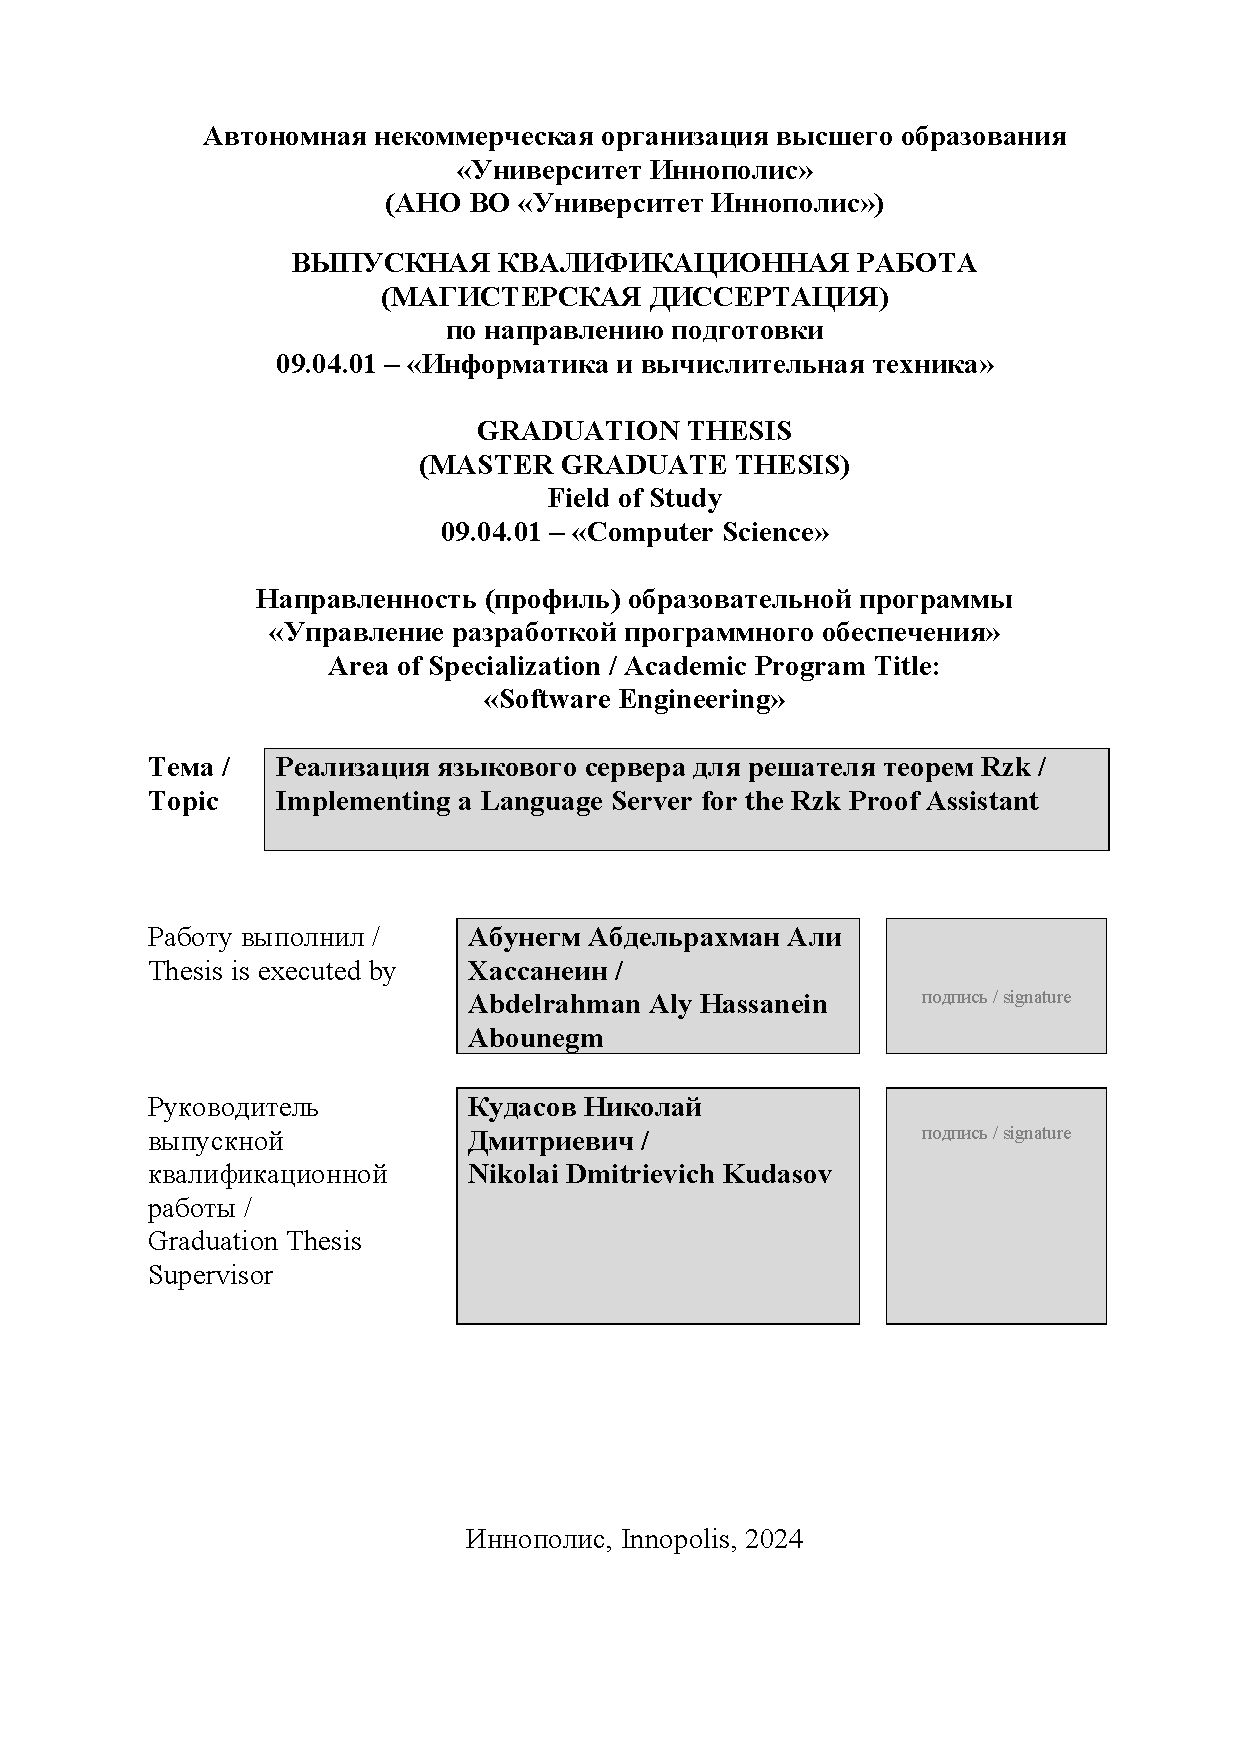
\includepdf[pages=-]{title.pdf}
\tableofcontents
\listoftables
\listoffigures


\newpage
\begin{abstract}
  The Riehl-Shulman type theory for synthetic $\infty$-categories is a new theory building on Homotopy Type Theory (HoTT).
  The experimental proof assistant \Rzk{} offers an automated proof checker for this theory.
  With the goal of making this theory more accessible to mathematicians and computer scientists,
  we present in this paper a work-in-progress on a collection of command line and interactive tools for \Rzk.
  These tools comprise a language server, an accompanying Visual Studio Code (VS Code) extension,
  and a list of smaller satellite tools offering minor conveniences.
  Although we focus on the support of VS Code,
  the language server is also compatible with other popular editors that support the Language Server Protocol (LSP),
  such as Emacs and Vim.

  % To support interactivity, we adjust the typechecker in \Rzk{} to work in an incremental fashion. In this paper, we present an initial version of a generic approach to the design of typecheckers that focus on LSP support. Building on top of this, we design and implement the language server for \Rzk. The language server offers advanced language features, including syntax and semantic highlighting, code completion, and diagnostics reporting. The VS Code extension complements the server with a user-friendly interface, facilitating interactive theorem proving and exploration of higher-dimensional structures.

  % Additional tools are developed along with the extension and language server to provide a pleasant experience outside the editor as well. These include a plugin to MkDocs that renders tope diagrams, a GitHub Action to type-check formalizations in Continuous integration environments, and a Pygments plugin for syntax highlighting \Rzk{} code blocks in LaTeX documents.

  % The effectiveness and usability of the language server and satellite tools is verified by \Rzk{} users coming from different backgrounds (mathematics, computer science, and software engineering), who use \Rzk{} to formalize theorems and provide feedback on their experience.
\end{abstract}

\setcounter{page}{8} % set manually an actual number from which introduction starts
\chapter{Introduction}
\label{chap:intro}
\chaptermark{Optional running chapter heading}
\section{Spacing \& Type}
\label{sec:section}

This is a section. This is a citation without brackets. and this is one with brackets \cite{A}. Multiple \cite{A,B,C} Here's a reference to a subsection: \ref{sec:subsection}. Citation of an online article \cite{D}. Citation of an online proceeding \cite{F}. The body of the text and abstract must be double-spaced except for footnotes or long quotations. Fonts such as Times Roman, Bookman, New Century Schoolbook, Garamond, Palatine, and Courier are acceptable and commonly found on most computers. The same type must be used throughout the body of the text. The font size must be 10 point or larger and footnotes\footnote{This is a footnote.} must be two sizes smaller than the text\footnote{This is another footnote.} but no smaller than eight points. Chapter, section, or other headings should be of a consistent font and size throughout the ETD, as should labels for illustrations, charts, and figures.

\subsection{Creating a Subsection}
\label{sec:subsection}

\subsubsection{Creating a Subsubsection}
\subsubsection{Creating a Subsubsection}
\subsubsection{Creating a Subsubsection}

\paragraph{This is a heading level below subsubsection}

And this is a quote: 
%
\begin{quote}
\blindtext
\end{quote}

\begin{figure}[hbt]
\centering

\includegraphics[]{figs/inno.png}
\caption{One kernel at $x_s$ (\emph{dotted kernel}) or two kernels at
$x_i$ and $x_j$ (\textit{left and right}) lead to the same summed estimate
at $x_s$. This shows a figure consisting of different types of
lines. Elements of the figure described in the caption should be set in
italics, in parentheses, as shown in this sample caption.}
\label{fig:example}
\end{figure}

This is a table:
% currsize is not set in the long table environment, so we need to set it before we set it up.
\makeatletter
\let\@currsize\normalsize
\makeatother

% tabular environments are set to be single-spaced in the  thesis class,  but long tables do not use tabular
% to get around this, set the spacing to single spacing at the start of the long table environment, and set it back to double-spacing at the end of it

\begin{longtable}{c|c|c}
\caption[This is the title I want to appear in the List of Tables]{This Is a Table Example} \label{tab:pfams} \\
\hline
A & B & C \\
\hline
\endfirsthead
\multicolumn{3}{@{}l}{} \\
\hline
A & B & C\\
\hline
\endhead
a1 & b1 & c1 \\
a2 & b2 & c2\\
a3 & b3 & c3\\
a4 & b4 & c4\\
\hline
\end{longtable}

The package ``upgreek'' allows us to use non-italicized lower-case greek letters. See for yourself: $\upbeta$, $\bm\upbeta$, $\beta$, $\bm\beta$. Next is a numbered equation:
\begin{align}
\label{eq:name}
\|\bm{X}\|_{2,1}={\underbrace{\sum_{j=1}^nf_j(\bm{X})}_{\text{convex}}}=\sum_{j=1}^n\|\bm{X}_{.,j}\|_2
\end{align}
The reference to equation (\ref{eq:name}) is clickable. 
\section[Theorems, Corollaries, Lemmas, Proofs, Remarks, Definitions and Examples]{Theorems, Corollaries, Lemmas, Proofs, Remarks, Definitions,and Examples}

\begin{theorem}
\label{thm:onlytheorem}
\blindtext
\end{theorem}

\begin{proof}
I'm a (very short) proof.
\end{proof}

\begin{lemma}
I'm a lemma.
\end{lemma}

\begin{corollary}
I include a reference to Thm. \ref{thm:onlytheorem}.
\end{corollary}

\begin{proposition}
I'm a proposition.
\end{proposition}

\begin{remark}
I'm a remark. 
\end{remark}

\begin{definition}
I'm a definition. I'm a definition. I'm a definition. I'm a definition. I'm a definition. I'm a definition. I'm a definition. I'm a definition. I'm a definition. I'm a definition. I'm a definition. 
\end{definition}

\begin{example}
I'm an example.
\end{example}


\section[Optional table of contents heading]{Section with\\ linebreaks in\\the
name}


\Blindtext[2]





\chapter{Literature Review}
\label{chap:lr}
\chaptermark{Second Chapter Heading}

\section{Language Server Protocol}

The Language Server Protocol is a common protocol for programming language analyzers to communicate with development tools. The Language Server Protocol is used between a tool (the client) and a language smartness provider (the server) to integrate features like auto complete, go to definition, find all references and alike into the tool. The Language Server Protocol is used by many development tools like Visual Studio Code, Eclipse, Emacs, Sublime Text, Atom, and Vim. The Language Server Protocol is developed by Microsoft and is released under the Creative Commons Attribution License.

Its development started on June 27, 2016.
Microsoft collaborated with Red Hat and Codenvy to standardize the protocol's specifictation.
% https://www.infoworld.com/article/3088698/microsoft-backed-langauge-server-protocol-strives-for-language-tools-interoperability.html
% https://sdtimes.com/che/codenvy-microsoft-red-hat-collaborate-language-server-protocol/

\subsection{SLSP}

LSP is not good enough for "specification languages" (SL) because it is not designed for them. SLSP is a protocol for specification languages based on LSP.

It adds missing features (requests and notification types) for specification languages. It also adds a new feature for specification languages: "proof view" (a view of the proof state - like Lean's Info View).

% TODO: figure out what it uses DAP for exactly.

\section{Proof Assistants}

\chapter{System Requirements and Design}
\label{chap:met}

\chapter{Implementation}
\label{chap:impl}

\section{\Rzk{} Language Server and VS Code extesion}

In this section, we describe design and implementation of the language server
and the VS Code extension for \Rzk{} proof assistant.
The language server has direct access to the proof assistant internals,
including the typechecking algorithm and the internal abstract syntax representation,
and provides an interface conforming to the Language Server Protocol.
The VS Code extension then acts as a buffer between the editor (VS Code)
and the language server, to bring the interactive capabilities to the user.

We subject the language server to support the features specified below.

\subsubsection{Intuitive Interface and Syntax Highlighting.}

The VS Code extension introduces an intuitive interface that aligns with
the expectations of mathematicians and computer scientists.
Users benefit from clear and accessible navigation,
enabling efficient exploration of HoTT-based structures.
Furthermore, the extension provides syntax and semantic highlighting,
enhancing code readability, and facilitating error detection.

\subsubsection{Code Completion and Suggestions.}

\Rzk{}'s VS Code extension leverages the LSP to offer intelligent code completion
and context-aware suggestions. As users work with \Rzk{}, the extension assists
in writing code more efficiently by providing relevant suggestions, reducing
the likelihood of syntax errors, and accelerating the development process.

\subsubsection{Real-time Error Checking.}

One of the extension's notable strengths lies in its ability to perform real-time error checking.
As users input and modify code, the language server continuously analyzes it,
reporting back any type errors or other issues with the proof.
This proactive error checking mechanism empowers users to identify and rectify issues promptly,
fostering the creation of mathematically sound programs.

\subsection{VS Code extension}

To bring about these features to the users, a thin wrapper around the language server in the form of a VS Code extension is necessary.
Additionally, the extension manages the installation of the language server itself on all major operating systems (Windows, macOS, and Ubuntu)
powered by pre-built binaries attached to releases on GitHub,
in addition to facilitating building the language server from source on platforms
for which pre-built binaries are not available.
It is also worth mentioning that the language server is designed to be compatible
with any other editor that supports LSP.
In particular, users have reported success in integrating it with the NeoVim editor,
and it is planned to be tested with other editors as well.

\subsection{\Rzk{} Language Server}

At the core of the \Rzk{} tool suite is the language server that powers all the editor features that make it pleasant to develop proofs in \Rzk{}. In particular, it currently supports semantic highlighting, diagnostic messages, and text completion. Additionally, progress reporting for long-running processes (such as type-checking for large projects) is currently under work.

For the first versions of the language server, it is shipped as part of the \Rzk{} proof assistant itself under a different subcommand, but it is planned to decouple both components and have the language server depend on the core library. They are implemented in the Haskell programming language using the \texttt{lsp}\footnote{\url{https://hackage.haskell.org/package/lsp}} package.

\chapter{Evaluation and Discussion}
\label{chap:eval}

\chapter{Conclusion}
\label{chap:conclusion}



%% REFERENCES
\printbibliography[heading=bibintoc,title={Bibliography cited}]
\appendix
\chapter{Extra Stuff}
\blindtext

\chapter{Even More Extra Stuff}
\blindtext

\end{document}
